\documentclass{beamer}

\usepackage{tikz-uml}
\usepackage[T1]{fontenc}
\usepackage{listings}
\usepackage{amsmath}
\usepackage{verbatim}
\usepackage{tikz-uml}
\usepackage{ifthen}
\usetikzlibrary {automata,positioning}
\usepackage{xargs}
\newcommand{\semaut}[1]{[\![#1]\!]}
\newcommand{\sembox}[1]{
    #1
}
\newcommandx{\automaton}[7][1=, 2=Q, 3=C, 4=\Delta, 5=\Sigma, 6=s, 7=F]{
    (#2#1, #3#1, #4#1, #5, #6#1, #7#1)
}
\newcommandx{\transition}[6][1=, 2=q, 3=q', 4=\phi, 5=p, 6=a]{
    (#2#1, #4#1, #5#1, #6, #3#1)
}
\newcommandx{\clockreduction}[0]{
    \mathbb{C}_r
}
\newcommandx{\deadedge}[0]{
    \mathbb{T}_d
}
\newcommandx{\deadclock}[0]{
    \mathbb{C}_d
}
\newcommandx{\deadstate}[0]{
    \mathbb{S}_d
}
\newcommandx{\unreachable}[0]{
    \mathbb{S}_u
}
\newcommandx{\pruning}[0]{
    \mathbb{P}
}
\newcommandx{\str}[1]{
    \underline{#1}
}

\newcommandx{\plot}[8]{
    \begin{tikzpicture}
        \begin{semilogyaxis}[
                title={Mean Time},
                width=15cm,
                height=10cm,
                ymin=0,
                legend pos=north west,
                xlabel={Iterations},
                ylabel={Time(ns)},
                xtick={#1},
                ymajorgrids=true,
            ]

            \addplot[color=yellow, mark=square*] coordinates {#2};
            \addlegendentry{N}
            \addplot[color=gray, mark=square*] coordinates {#3};
            \addlegendentry{E}
            \addplot[color=red, mark=square*] coordinates {#4};
            \addlegendentry{S}
            \addplot[color=black, mark=square*] coordinates {#5};
            \addlegendentry{SS}
            \addplot[color=green, mark=square*] coordinates {#6};
            \addlegendentry{SE}
            \addplot[color=violet, mark=square*] coordinates {#7};
            \addlegendentry{ES}
            \addplot[color=blue, mark=square*] coordinates {#8};
            \addlegendentry{EE}
        \end{semilogyaxis}
    \end{tikzpicture}
}

\newcommandx{\plotmem}[8]{
    \begin{tikzpicture}
        \begin{semilogyaxis}[
                title={Allocated Memory},
                width=15cm,
                height=10cm,
                ymin=0,
                legend pos=north west,
                xlabel={Iterations},
                ylabel={Memory (kb)},
                xtick={#1},
                ymajorgrids=true,
            ]

            \addplot[color=yellow, mark=square*] coordinates {#2};
            \addlegendentry{N}
            \addplot[color=gray, mark=square*] coordinates {#3};
            \addlegendentry{E}
            \addplot[color=red, mark=square*] coordinates {#4};
            \addlegendentry{S}
            \addplot[color=black, mark=square*] coordinates {#5};
            \addlegendentry{SS}
            \addplot[color=green, mark=square*] coordinates {#6};
            \addlegendentry{SE}
            \addplot[color=violet, mark=square*] coordinates {#7};
            \addlegendentry{ES}
            \addplot[color=blue, mark=square*] coordinates {#8};
            \addlegendentry{EE}
        \end{semilogyaxis}
    \end{tikzpicture}
}
\newcommandx{\captionof}[2]{

}

\newcommand{\name}{}

\addtobeamertemplate{navigation symbols}{}{%
    \usebeamerfont{footline}%
    \usebeamercolor[fg]{footline}%
    \hspace{1em}%
    \name
    \hspace{1em}%
    \insertframenumber/\inserttotalframenumber
}

\definecolor{bluekeywords}{rgb}{0,0,1}
\definecolor{greencomments}{rgb}{0,0.5,0}
\definecolor{redstrings}{rgb}{0.64,0.08,0.08}
\definecolor{xmlcomments}{rgb}{0.5,0.5,0.5}
\definecolor{types}{rgb}{0.17,0.57,0.68}

\lstdefinestyle{csharp}{language=[Sharp]C,
    captionpos=b,
    %numbers=left, %Nummerierung
    %numberstyle=\tiny, % kleine Zeilennummern
    frame=lines, % Oberhalb und unterhalb des Listings ist eine Linie
    showspaces=false,
    showtabs=false,
    breaklines=true,
    showstringspaces=false,
    breakatwhitespace=true,
    commentstyle=\color{greencomments},
    morekeywords={partial, var, value, get, set},
    keywordstyle=\color{bluekeywords},
    stringstyle=\color{redstrings},
    basicstyle=\ttfamily\tiny,
}

\usetheme{Frankfurt}
\useinnertheme{rectangles}
% \setbeamertemplate{footline}[frame number]


\title{TREAT}
\subtitle{Timed Regular Expression to Automaton Transformation}
\author{Group 30}
\institute{Aalborg Universitet}
\date{2024}

\begin{document}


\frame{\titlepage}

\begin{frame}{Agenda}
    \tableofcontents
\end{frame}

\section{Intro} % each section gets own category on top bar, each frame within gets a subcategory
\renewcommand{\name}{Marcus}
%Marcus Section

\begin{frame}{Introduction}
    \centering
    \LARGE\textbf{TREAT} \\
    \vspace{0.5cm}
    \Large\textit{Timed Regular Expression to Automaton Transformation}
\end{frame}

\section{Process}

\begin{frame}{Process}
    \begin{itemize}
        \item Initial Problem
        \item Pivot
        \item Human Readability and Usability
    \end{itemize}
\end{frame}

\begin{frame}{Process}
    \textbf{Initial Problem}

    ``Better Timed Pattern Searching in Log Files''
    \newline
    \begin{itemize}
        \item The paper: ``Timed Regular Expressions''
        \item What should the program contain?
              \begin{itemize}
                  \item Parse TREs
                  \item Convert TREs to timed automata
                  \item Perform checking (Output to UPPAAL)
              \end{itemize}
    \end{itemize}

    Can we output to UPPAAL in a better way?
\end{frame}

\begin{frame}{Process}
    \textbf{Pivot}

    We will still have the same features, but checking will take a lower priority.
    \newline
    \begin{itemize}
        \item Pruning
        \item Graphing
    \end{itemize}
\end{frame}

\begin{frame}{Process}
    \textbf{Human Readability and Usability}

    Focus on efficient transformation from TRE to TA.
    \newline
    \begin{itemize}
        \item TRE input improvement
              \begin{itemize}
                  \item Multi-character symbols
              \end{itemize}
        \item CLI
        \item TikZ
    \end{itemize}

    These could have been done regardless, but became a larger focus now.
\end{frame}

\section{Tokenizer}

\begin{frame}[shrink=5]{Tokenizer}
    \begin{center}
        \scalebox{0.9}{
    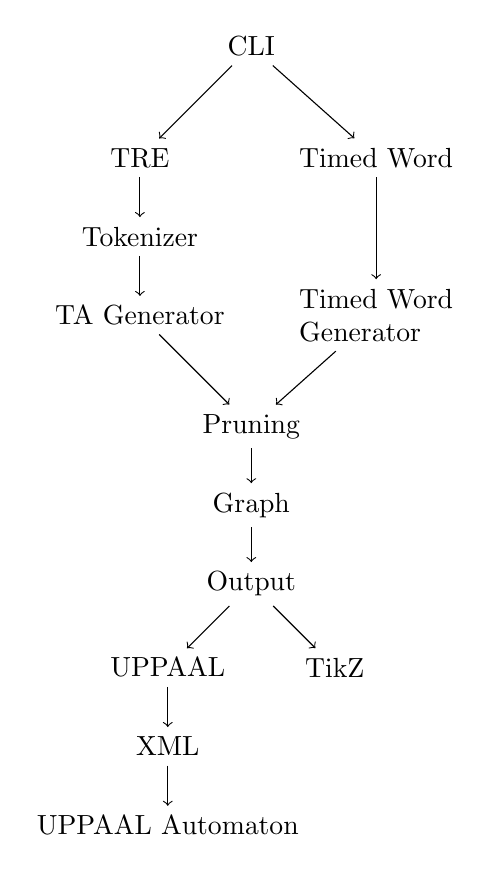
\begin{tikzpicture}[node distance = 1cm, auto]\label{fig:TREATdiagram}
        \node (CLI) {CLI};
        
        \node (TRE) [node distance = 2cm, below left of = CLI] {TRE};
        \node (TimedWord) [node distance = 3cm, right of = TRE] {Timed Word};
        \node (Tokenizer) [below of = TRE] {Tokenizer};
        \node (TAGenerator) [below of = Tokenizer] {TA Generator};
        \node (Pruning) [node distance = 2cm, below right of = TAGenerator] {Pruning};
        \node (Graph) [below of = Pruning] {Graph};
        \node (Output) [below of = Graph] {Output};
        \node (UPPAAL) [node distance = 1.5cm, below left of = Output] {UPPAAL};
        \node (XML) [below of = UPPAAL] {XML};
        \node (UPPAALAutomaton) [below of = XML] {UPPAAL Automaton};
        \node (TikZ) [node distance = 1.5cm, below right of = Output] {TikZ};
        \node (TimedWordGenerator) [node distance = 3cm, right of = TAGenerator,  align=left] {Timed Word\\Generator};
    
        \draw[->] (CLI) -- (TRE);
        \draw[->] (TRE) -- (Tokenizer);
        \draw[->] (Tokenizer) -- (TAGenerator);
        \draw[->] (TAGenerator) -- (Pruning);
        \draw[->] (Pruning) -- (Graph);
        \draw[->] (Graph) -- (Output);
        \draw[->] (Output) -- (UPPAAL);
        \draw[->] (UPPAAL) -- (XML);
        \draw[->] (XML) -- (UPPAALAutomaton);
        \draw[->] (Output) -- (TikZ);
        \draw[->] (CLI) -- (TimedWord);
        \draw[->] (TimedWord) -- (TimedWordGenerator);
        \draw[->] (TimedWordGenerator) -- (Pruning);
    \end{tikzpicture}
}

    \end{center}
\end{frame}

\begin{frame}[shrink=20]{Parser}
    
\textbf{CFG}

TimedRegex := Rename

\qquad	$\mid$ $\epsilon$

Rename := Intersection renameStart RenameSymbols renameEnd

\qquad $\mid$ Intersection

RenameSymbols := match match renameSeparator RenameSymbols

\qquad $\mid$ match match

Intersection := Union intersection Intersection

\qquad $\mid$ Union

Union := Concatenation union Union

\qquad $\mid$ Concatenation

Concatenation := Interval Concatenation

\qquad $\mid$ Interval absorb Concatenation

\qquad $\mid$ Interval

Concatenation := Concatenation Interval

\qquad $\mid$ Interval

Interval := Unary IntervalStartEnd Number intervalSeperator Number IntervalStartEnd

\qquad $\mid$ Unary

IntervalStartEnd := intervalOpen

\qquad $\mid$ intervalClose

Number := digit Number

\qquad $\mid$ digit

Unary := Match guaranteedIterator

\qquad $\mid$ Match guaranteedIterator absorb

\qquad $\mid$ Match iterator

\qquad $\mid$ Match iterator absorb

\qquad $\mid$ Match

Match := parenthesisStart Rename parenthesisEnd

\qquad $\mid$ match

\qquad $\mid$ matchAny


\end{frame}

\begin{frame}[shrink=10]{Parser}
    \begin{center}
        \scalebox{0.8}{\begin{tikzpicture}
    %interfaces
    \umlclass[x=0,y=-3]{IAstNode}{token: Token}{}

    %classes
    \umlclass[x=0,y=-6]{IBinary}{left: IAstNode}{right: IAstNode}
    \umlclass[x=3.5,y=-6]{IUnary}{child: IAstNode}{}
    \umlclass[x=6.5,y=-6]{Match}{}{}
    %\umlclass[anchor=north,x=1,y=-9]{Interval}{startInterval: int\\endInterval: int\\startInclusive: bool\\endInclusive: bool}{}
    %\umlclass[anchor=north,x=6,y=-9]{Rename}{renameSymbols: symbolReplace[]}{}
    \umlclass[x=9,y=-6]{Epsilon}{}{}
    \umlsimpleclass[x=3.5,y=-8,draw=none,fill=none,alias=unarydots,scale=2]{...}
    \umlsimpleclass[x=3.5,y=-8,fill=none,draw=none,alias=phantomunary]{ }
    \umlsimpleclass[x=0,y=-8,fill=none,draw=none,scale=2]{...}
    \umlsimpleclass[x=0,y=-8,fill=none,draw=none,alias=phantombinary]{ }

    % \umlclass[anchor=north,x=9,y=-12]{AbsorbedConcatenation}{}{}
    % \umlclass[anchor=north,x=12,y=-12]{AbsorbedGuaranteedIterator}{}{}
    % \umlclass[anchor=north,x=15,y=-12]{AbsorbedIterator}{}{}
    % \umlclass[anchor=north,x=18,y=-12]{Concatenation}{}{}
    % \umlclass[anchor=north,x=21,y=-12]{GuaranteedIterator}{}{}
    % \umlclass[anchor=north,x=27,y=-12]{Intersection}{}{}
    % \umlclass[anchor=north,x=6,y=-12]{Interval}{}{}
    % \umlclass[anchor=north,x=3,y=-12]{Iterator}{}{}
    % \umlclass[anchor=north,x=0,y=-12]{Union}{}{}
    

    %transitions
    \umlVHVinherit[arm1=1.5cm]{IUnary}{IAstNode}
    \umlVHVinherit[]{IBinary}{IAstNode}
    \umlVHVinherit[arm1=1.5cm]{Match}{IAstNode}
    \umlVHVinherit[arm1=1.5cm]{Epsilon}{IAstNode}
    \umlVHVinherit[arm1=0.5cm]{phantomunary}{IUnary}
    \umlVHVinherit[arm1=0.5cm]{phantombinary}{IBinary}

    % \umlaggreg[attr1=1|,attr2=2|]{IBinary}{IAstNode}

    % \umlVHVinherit[]{Interval}{IUnary}
    % \umlVHVinherit[]{Rename}{IUnary}

    %\draw [tikzuml aggregation style] (IUnary.-120)-- ++(0cm,-1cm)node[pos=0.2, left]{1} -- ++(-4.5cm,0cm) |- (IAstNode.west)node[pos=0.8, below]{1};

\end{tikzpicture}}
    \end{center}
\end{frame}

\section{TA}
\begin{frame}[shrink=5]{TA}
    \begin{center}
        \scalebox{0.9}{
    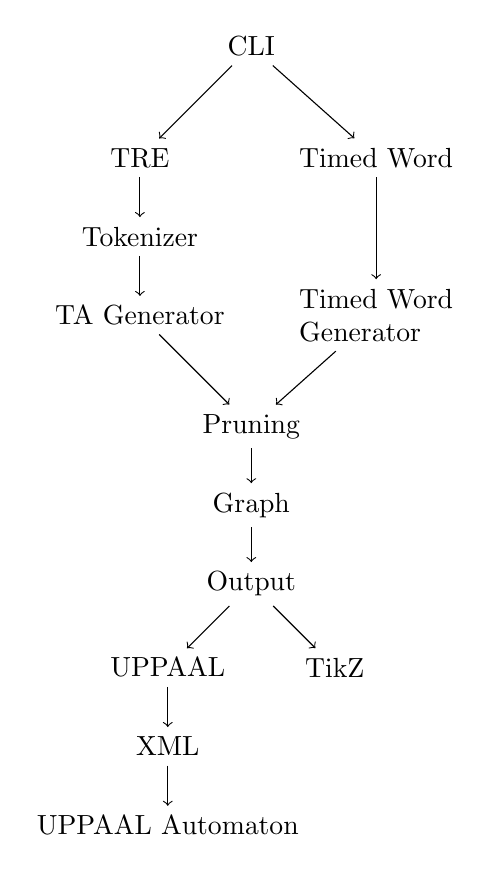
\begin{tikzpicture}[node distance = 1cm, auto]\label{fig:TREATdiagram}
        \node (CLI) {CLI};
        
        \node (TRE) [node distance = 2cm, below left of = CLI] {TRE};
        \node (TimedWord) [node distance = 3cm, right of = TRE] {Timed Word};
        \node (Tokenizer) [below of = TRE] {Tokenizer};
        \node (TAGenerator) [below of = Tokenizer] {TA Generator};
        \node (Pruning) [node distance = 2cm, below right of = TAGenerator] {Pruning};
        \node (Graph) [below of = Pruning] {Graph};
        \node (Output) [below of = Graph] {Output};
        \node (UPPAAL) [node distance = 1.5cm, below left of = Output] {UPPAAL};
        \node (XML) [below of = UPPAAL] {XML};
        \node (UPPAALAutomaton) [below of = XML] {UPPAAL Automaton};
        \node (TikZ) [node distance = 1.5cm, below right of = Output] {TikZ};
        \node (TimedWordGenerator) [node distance = 3cm, right of = TAGenerator,  align=left] {Timed Word\\Generator};
    
        \draw[->] (CLI) -- (TRE);
        \draw[->] (TRE) -- (Tokenizer);
        \draw[->] (Tokenizer) -- (TAGenerator);
        \draw[->] (TAGenerator) -- (Pruning);
        \draw[->] (Pruning) -- (Graph);
        \draw[->] (Graph) -- (Output);
        \draw[->] (Output) -- (UPPAAL);
        \draw[->] (UPPAAL) -- (XML);
        \draw[->] (XML) -- (UPPAALAutomaton);
        \draw[->] (Output) -- (TikZ);
        \draw[->] (CLI) -- (TimedWord);
        \draw[->] (TimedWord) -- (TimedWordGenerator);
        \draw[->] (TimedWordGenerator) -- (Pruning);
    \end{tikzpicture}
}

    \end{center}
\end{frame}
\begin{frame}[shrink=10]{TA UML}
    \begin{center}
        \begin{tikzpicture}
    \umlclass{TA}{clockCount: int\\edges/locations}{}
    
    \umlclass[x=-4, y=-4]{Location}{id: int\\initial: bool\\}{}
    \umlcompo[geometry=|-|,attr1=0..*|,attr2=1|,pos1=1.8,pos2=0.2]{TA}{Location}
    
    \umlclass[y=-4]{Edge}{id: int\\ranges\\resetClocks}{}
    \umlcompo[geometry=|-|,attr1=|0..*,attr2=1|,pos1=1.8,pos2=0.2]{TA}{Edge}
    \umlassoc{Edge}{Location}

    \umlclass[x=4,y=-4]{Clock}{id: int}{}
    \umlcompo[geometry=|-|,attr1=|0..*,attr2=1|,pos1=1.8,pos2=0.2]{TA}{Edge}
    \umlassoc{Edge}{Clock}
    
\end{tikzpicture}
    \end{center}
\end{frame}

%End of Marcus section

\renewcommand{\name}{Frederik}
% =======================================================================
% Semantics
% =======================================================================

\section{TA Generator}
\begin{frame}[shrink=5]{TA Generator}
    \begin{center}
        \scalebox{0.9}{
    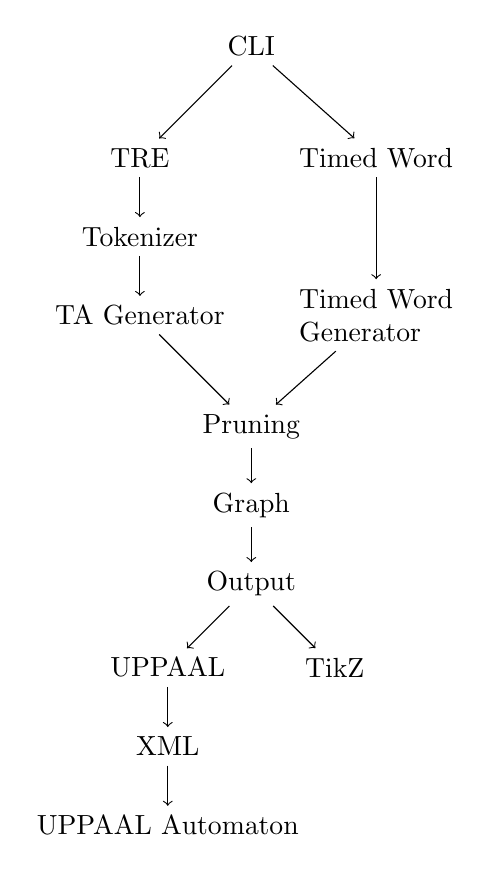
\begin{tikzpicture}[node distance = 1cm, auto]\label{fig:TREATdiagram}
        \node (CLI) {CLI};
        
        \node (TRE) [node distance = 2cm, below left of = CLI] {TRE};
        \node (TimedWord) [node distance = 3cm, right of = TRE] {Timed Word};
        \node (Tokenizer) [below of = TRE] {Tokenizer};
        \node (TAGenerator) [below of = Tokenizer] {TA Generator};
        \node (Pruning) [node distance = 2cm, below right of = TAGenerator] {Pruning};
        \node (Graph) [below of = Pruning] {Graph};
        \node (Output) [below of = Graph] {Output};
        \node (UPPAAL) [node distance = 1.5cm, below left of = Output] {UPPAAL};
        \node (XML) [below of = UPPAAL] {XML};
        \node (UPPAALAutomaton) [below of = XML] {UPPAAL Automaton};
        \node (TikZ) [node distance = 1.5cm, below right of = Output] {TikZ};
        \node (TimedWordGenerator) [node distance = 3cm, right of = TAGenerator,  align=left] {Timed Word\\Generator};
    
        \draw[->] (CLI) -- (TRE);
        \draw[->] (TRE) -- (Tokenizer);
        \draw[->] (Tokenizer) -- (TAGenerator);
        \draw[->] (TAGenerator) -- (Pruning);
        \draw[->] (Pruning) -- (Graph);
        \draw[->] (Graph) -- (Output);
        \draw[->] (Output) -- (UPPAAL);
        \draw[->] (UPPAAL) -- (XML);
        \draw[->] (XML) -- (UPPAALAutomaton);
        \draw[->] (Output) -- (TikZ);
        \draw[->] (CLI) -- (TimedWord);
        \draw[->] (TimedWord) -- (TimedWordGenerator);
        \draw[->] (TimedWordGenerator) -- (Pruning);
    \end{tikzpicture}
}

    \end{center}
\end{frame}
\begin{frame}[fragile]{Match semantics}
    \begin{definition}
        Assarin et al.
        
        The automaton for \underline{$[\![a]\!]$}, $a\in\Sigma$ is $(\{s,f\},\emptyset,\Delta,\Sigma,s,\{f\})$ where the transition relation is $\Delta={(s,true,\emptyset,a,f)}$.
    \end{definition}
        
    \begin{lstlisting}[style=csharp,basicstyle=\small]
void Visit(Match match)
{
    TimedAutomaton ta = new(_regex);
    
    State initial = ta.AddState(newInitial: true);
    State final = ta.AddState(true);

    ta.AddEdge(initial, final, match.Token.Match);

    _stack.Push(ta);
}
    \end{lstlisting}
\end{frame}

\begin{frame}{Union semantics}
    Assarin et al.

    \textit{The automaton for $[[\varphi_1\vee\varphi_2]]$ is $(Q_1\cup Q_2 \cup \{s\},C_1\cup C_2,\Delta,\Sigma,s,F_1\cup F_2)$, where $\Delta$ is constructed
        by adding to $\Delta_1\cup \Delta_2$ two new $\epsilon$-transitions $(s, x = 0,\emptyset,\epsilon,s_i)$, where $x$ is any clock and $i\in{1,2}$
        (if there is no clock in the automata we should add one).}

    \usetikzlibrary {automata,positioning}
% "A|B"
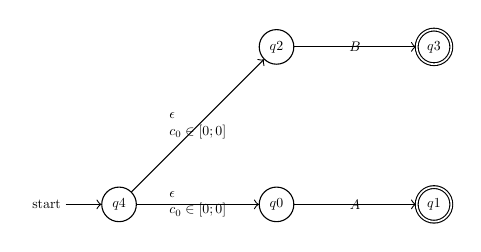
\begin{tikzpicture}[every node/.style={scale=0.5}]
    \node[state] at (2, 0)(q0){$q0$};
    \node[state, accepting] at (4, 0)(q1){$q1$};
    \node[state] at (2, 2)(q2){$q2$};
    \node[state, accepting] at (4, 2)(q3){$q3$};
    \node[state, initial] at (0, 0)(q4){$q4$};
    
    \path[->]
        (q0)edge node[align=left]{$A$}(q1)
        (q2)edge node[align=left]{$B$}(q3)
        (q4)edge node[align=left]{$\epsilon$\\$c_0\in[0;0]$}(q0)
        (q4)edge node[align=left]{$\epsilon$\\$c_0\in[0;0]$}(q2)
        ;
\end{tikzpicture}
    
% "A|B"
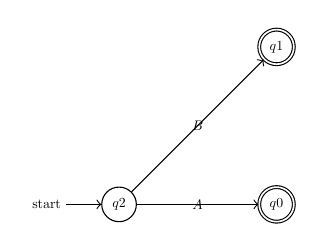
\begin{tikzpicture}[every node/.style={scale=0.5}]
    \node[state, accepting] at (2, 0)(q0){$q0$};
    \node[state, accepting] at (2, 2)(q1){$q1$};
    \node[state, initial] at (0, 0)(q2){$q2$};
    
    \path[->]
        (q2)edge node[align=left]{$A$}(q0)
        (q2)edge node[align=left]{$B$}(q1)
        ;
\end{tikzpicture}
\end{frame}

\begin{frame}{Union semantics revised}
    % We can improve upon union by removing unnecessary epsilon transitions.
\begin{definition}
    Union\label{def:union-semantics}
    
    \sembox{
        $\semaut{\varphi_1|\varphi_2}=
        \left\{\begin{array}{ll}
            \semaut{(\epsilon\cdot\varphi_1)\cup\varphi_2} & if (q_1,\phi_1,p_1,a,s_1)\in\Delta_1 \\
            \semaut{\varphi_1\cup(\epsilon\cdot\varphi_2)} & if (q_2,\phi_2,p_2,a,s_2)\in\Delta_2 \\
            \automaton & otherwise \\
        \end{array}\right.
        $
        
        Where
        
        $f\transition=
        \left\{\begin{array}{ll}
            \transition[][s] & if q\in\{s_1,s_2\} \\
            \transition & otherwise \\
        \end{array}\right.
        $
        
        $Q=Q_1\cup Q_2 \cup {s}\backslash\{s_1,s_2\}$
        
        $C=C_1\cup C_2$
        
        $\Delta=f(\Delta_1\cup\Delta_2)$
        
        $F=F_1\cup F_2\backslash\{s_1,s_2\}$
    }
\end{definition}
\end{frame}

\begin{frame}[fragile]{Union implementation}
    \begin{lstlisting}[style=csharp,basicstyle=\tiny]
(TimedAutomaton right, TimedAutomaton left) = (_stack.Pop(), _stack.Pop());
EpsilonConcat(right);
EpsilonConcat(left);
TimedAutomaton ta = new(left, right, e => IsNotInitial(e.From), IsNotInitial);

State initial = ta.AddState(newInitial: true);

foreach (Edge edges in left.GetEdgesFrom(left.InitialState!)
    .Concat(right.GetEdgesFrom(right.InitialState!)))
{
    Edge e = ta.AddEdge(initial, edges.To, edges.Symbol);
    e.AddClockRanges(edges.GetClockRanges());
    e.AddClockResets(edges.GetClockResets());
}

static void EpsilonConcat(TimedAutomaton ta)
{
    if (ta.GetEdgesTo(ta.InitialState!).Any())
    {
        State oldInitial = ta.InitialState!;
        State newInitial = ta.AddState(ta.IsFinal(oldInitial), true);
        Edge edge = ta.AddEdge(newInitial, oldInitial, "\0");
    }
}
    \end{lstlisting}
\end{frame}

\begin{frame}[fragile]{Lazy intersection}
    Lazily generate new states
    \begin{lstlisting}[style=csharp,basicstyle=\tiny]
State GetNewState(State lState, State rState)
{
    if (!newLocs.TryGetValue((lState, rState), out State? state))
    {
        state = ta.AddState();
        newLocs[(lState, rState)] = state;
    }

    return state;
}
    \end{lstlisting}
\end{frame}

% =======================================================================
% Timed word generator
% =======================================================================
\section{Timed words}
\begin{frame}[shrink=5]{Timed words}
    \begin{center}
        \scalebox{0.9}{
    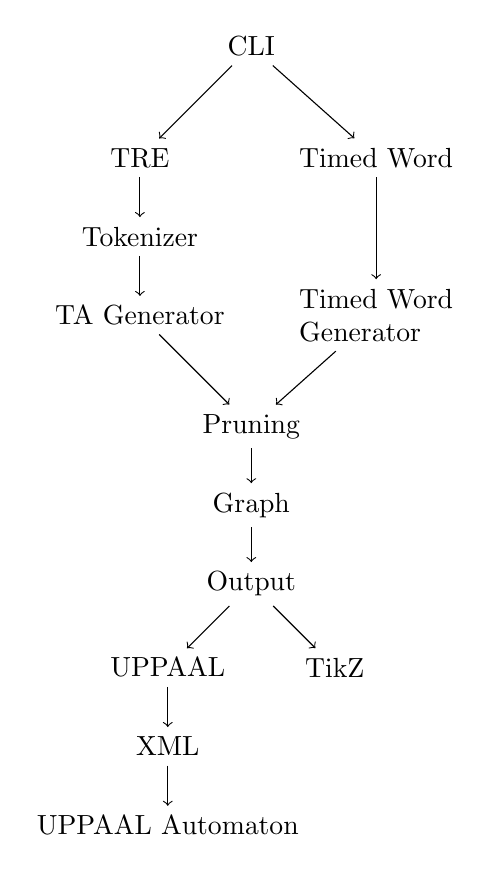
\begin{tikzpicture}[node distance = 1cm, auto]\label{fig:TREATdiagram}
        \node (CLI) {CLI};
        
        \node (TRE) [node distance = 2cm, below left of = CLI] {TRE};
        \node (TimedWord) [node distance = 3cm, right of = TRE] {Timed Word};
        \node (Tokenizer) [below of = TRE] {Tokenizer};
        \node (TAGenerator) [below of = Tokenizer] {TA Generator};
        \node (Pruning) [node distance = 2cm, below right of = TAGenerator] {Pruning};
        \node (Graph) [below of = Pruning] {Graph};
        \node (Output) [below of = Graph] {Output};
        \node (UPPAAL) [node distance = 1.5cm, below left of = Output] {UPPAAL};
        \node (XML) [below of = UPPAAL] {XML};
        \node (UPPAALAutomaton) [below of = XML] {UPPAAL Automaton};
        \node (TikZ) [node distance = 1.5cm, below right of = Output] {TikZ};
        \node (TimedWordGenerator) [node distance = 3cm, right of = TAGenerator,  align=left] {Timed Word\\Generator};
    
        \draw[->] (CLI) -- (TRE);
        \draw[->] (TRE) -- (Tokenizer);
        \draw[->] (Tokenizer) -- (TAGenerator);
        \draw[->] (TAGenerator) -- (Pruning);
        \draw[->] (Pruning) -- (Graph);
        \draw[->] (Graph) -- (Output);
        \draw[->] (Output) -- (UPPAAL);
        \draw[->] (UPPAAL) -- (XML);
        \draw[->] (XML) -- (UPPAALAutomaton);
        \draw[->] (Output) -- (TikZ);
        \draw[->] (CLI) -- (TimedWord);
        \draw[->] (TimedWord) -- (TimedWordGenerator);
        \draw[->] (TimedWordGenerator) -- (Pruning);
    \end{tikzpicture}
}

    \end{center}
\end{frame}
\begin{frame}[fragile]{Timed word generation}
    \begin{columns}
        \begin{column}{0.6\textwidth}
            nasa.gov
            \begin{lstlisting}[basicstyle=\tiny]
00 00 00 04 CDR
Roger. Clock.

00 00 00 13 CDR
Roger. We got a roll program.

00 00 00 15 CMP
Roger. Roll.

00 00 00 34 CDR
Roll's complete and the pitch is programed.

00 00 00 44 CDR
One Bravo.

00 00 01 02 CC
Apollo 11, Houston. You're good at 1 minute.
...
            \end{lstlisting}
        \end{column}
        \begin{column}{0.4\textwidth}
            apollo11transcript.csv
            \begin{lstlisting}[basicstyle=\tiny]
CDR, 4


CDR, 13


CMP, 15


CDR, 34


CDR, 44


CC, 62

...
            \end{lstlisting}
        \end{column}
    \end{columns}
\end{frame}

\begin{frame}[fragile]{Words as timed automata}
    In UPPAAL
    \begin{columns}
        \begin{column}{0.5\textwidth}
            % "(<CDR>|<CC>|<CMP>)+"
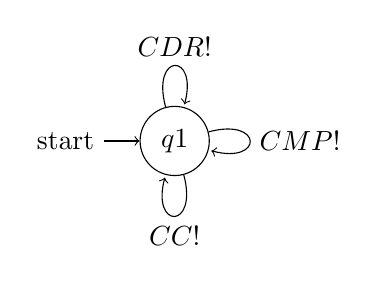
\begin{tikzpicture}[auto]
    \node[state, initial] at (0, 0)(q1){$q1$};
    
    \path[->]
        (q1)edge [loop above] node[align=left]{$CDR!$}(q1)
        (q1)edge [loop below] node[align=left]{$CC!$}(q1)
        (q1)edge [loop right] node[align=left]{$CMP!$}(q1)
        ;
\end{tikzpicture}

        \end{column}
        \begin{column}{0.5\textwidth}
            \begin{lstlisting}[basicstyle=\tiny]
update: index++
guard: index <= 8439 &&
    word[index] == "CDR" &&
    times[index] == c0
            \end{lstlisting}
        \end{column}
    \end{columns}
    \begin{lstlisting}[basicstyle=\tiny]
clock c0;
int32_t index = 0;
const string word[8439] = {"CDR", "CDR", "CMP", "CDR", "CDR", "CC", ... }
clock_t times[8439] = {4, 13, 15, 34, 44, 62, ... }
    \end{lstlisting}
\end{frame}

% =======================================================================
% Pruning
% =======================================================================
\section{Pruning}
\begin{frame}[shrink=5]{Pruning}
    \begin{center}
        \scalebox{0.9}{
    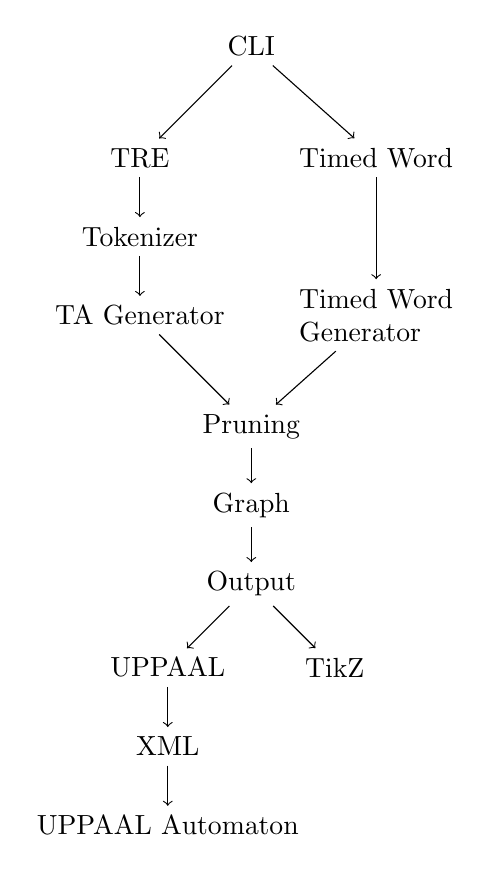
\begin{tikzpicture}[node distance = 1cm, auto]\label{fig:TREATdiagram}
        \node (CLI) {CLI};
        
        \node (TRE) [node distance = 2cm, below left of = CLI] {TRE};
        \node (TimedWord) [node distance = 3cm, right of = TRE] {Timed Word};
        \node (Tokenizer) [below of = TRE] {Tokenizer};
        \node (TAGenerator) [below of = Tokenizer] {TA Generator};
        \node (Pruning) [node distance = 2cm, below right of = TAGenerator] {Pruning};
        \node (Graph) [below of = Pruning] {Graph};
        \node (Output) [below of = Graph] {Output};
        \node (UPPAAL) [node distance = 1.5cm, below left of = Output] {UPPAAL};
        \node (XML) [below of = UPPAAL] {XML};
        \node (UPPAALAutomaton) [below of = XML] {UPPAAL Automaton};
        \node (TikZ) [node distance = 1.5cm, below right of = Output] {TikZ};
        \node (TimedWordGenerator) [node distance = 3cm, right of = TAGenerator,  align=left] {Timed Word\\Generator};
    
        \draw[->] (CLI) -- (TRE);
        \draw[->] (TRE) -- (Tokenizer);
        \draw[->] (Tokenizer) -- (TAGenerator);
        \draw[->] (TAGenerator) -- (Pruning);
        \draw[->] (Pruning) -- (Graph);
        \draw[->] (Graph) -- (Output);
        \draw[->] (Output) -- (UPPAAL);
        \draw[->] (UPPAAL) -- (XML);
        \draw[->] (XML) -- (UPPAALAutomaton);
        \draw[->] (Output) -- (TikZ);
        \draw[->] (CLI) -- (TimedWord);
        \draw[->] (TimedWord) -- (TimedWordGenerator);
        \draw[->] (TimedWordGenerator) -- (Pruning);
    \end{tikzpicture}
}

    \end{center}
\end{frame}
\begin{frame}{Example}
    $$C(A[5;10]\&(BA|A)[1;3])$$
    % Generated by: TimedRegex, Version = 1.0.0.0
% Date 5/14/2024 6:44:16 PM
\usetikzlibrary {automata,positioning}
\scalebox{0.9}{
    % "C(A[5;10]&(BA|A)[1;3])"
    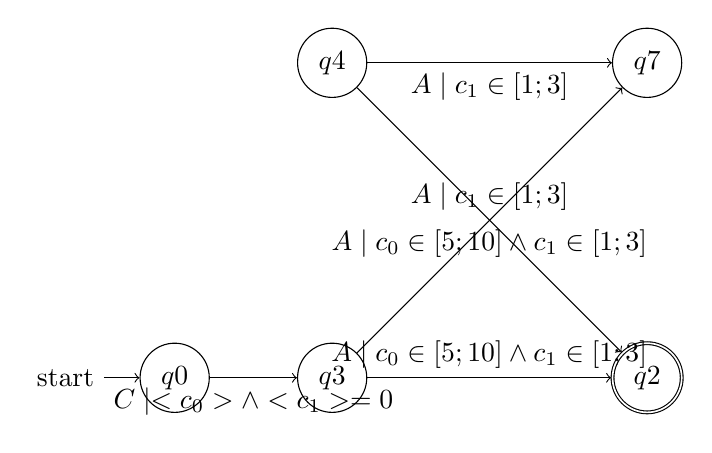
\begin{tikzpicture}[auto]
        \node[state, initial] at (0, 0)(q0){$q0$};
        \node[state] at (2, 0)(q3){$q3$};
        \node[state] at (2, 4)(q4){$q4$};
        \node[state] at (6, 4)(q7){$q7$};
        \node[state, accepting] at (6, 0)(q2){$q2$};
        
        \path[->]
            (q4)edge node[below]{$A\mid c_1\in[1;3]$}(q7)
            (q3)edge node[above]{$A\mid c_1\in[1;3]$}(q7)
            (q4)edge node[below]{$A\mid c_0\in[5;10]\wedge c_1\in[1;3]$}(q2)
            (q3)edge node[above]{$A\mid c_0\in[5;10]\wedge c_1\in[1;3]$}(q2)
            (q0)edge node[below]{$C\mid <c_0>\wedge<c_1>=0$}(q3)
            ;
    \end{tikzpicture}
}

\captionof{figure}{Lightly pruned automaton, to be used as an example.}
\label{fig:prune0}
\end{frame}
\begin{frame}{Clock reduction}
    Daws et al.
    % Generated by: TimedRegex, Version = 1.0.0.0
% Date 5/14/2024 6:44:16 PM
\usetikzlibrary {automata,positioning}
% "C(A[5;10]&(BA|A)[1;3])"
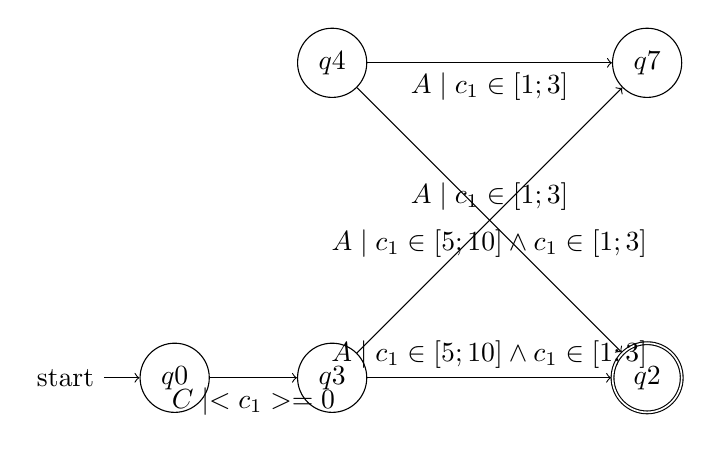
\begin{tikzpicture}[auto]
    \node[state, initial] at (0, 0)(q0){$q0$};
    \node[state] at (2, 0)(q3){$q3$};
    \node[state] at (2, 4)(q4){$q4$};
    \node[state] at (6, 4)(q7){$q7$};
    \node[state, accepting] at (6, 0)(q2){$q2$};
    
    \path[->]
        (q4)edge node[below]{$A\mid c_1\in[1;3]$}(q7)
        (q3)edge node[above]{$A\mid c_1\in[1;3]$}(q7)
        (q4)edge node[below]{$A\mid c_1\in[5;10]\wedge c_1\in[1;3]$}(q2)
        (q3)edge node[above]{$A\mid c_1\in[5;10]\wedge c_1\in[1;3]$}(q2)
        (q0)edge node[below]{$C\mid <c_1>=0$}(q3)
        ;
\end{tikzpicture}
 

\end{frame}
\begin{frame}{Dead transition}
    Pruning dead edges means pruning all edges that can never be taken because they are overconstrained.

We do this by first taking the intersection of all edges with multiple ranges.
If this intersection has no possible values we know the edge cannot possibly be taken.
Since it cannot be taken we can remove it.

Mathematically this can be described as a function ($\mathbb{E}$) taking in an automaton and returning a new automaton with the dead edges being pruned.

\sembox{
    $\deadedge(A)=\automaton[][Q][C][\Delta'][\Sigma][s][F]$
 
    $\Delta'=\{\transition\in\Delta\mid\phi\neq\emptyset\wedge\emptyset\neq\cap_{i=1}^n\phi_i\}$

}
    % Generated by: TimedRegex, Version = 1.0.0.0
% Date 5/14/2024 6:44:16 PM
\usetikzlibrary {automata,positioning}
\scalebox{0.9}{
    % "C(A[5;10]&(BA|A)[1;3])"
    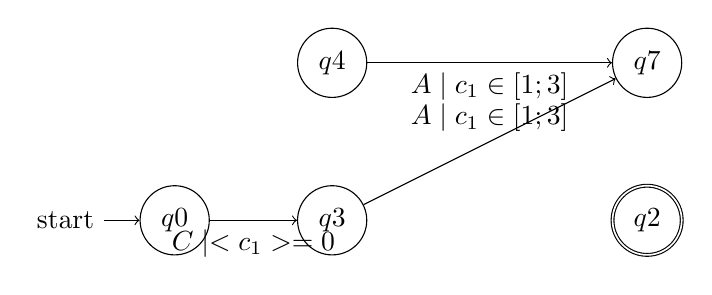
\begin{tikzpicture}[auto]
        \node[state, initial] at (0, 0)(q0){$q0$};
        \node[state] at (2, 0)(q3){$q3$};
        \node[state] at (2, 2)(q4){$q4$};
        \node[state] at (6, 2)(q7){$q7$};
        \node[state, accepting] at (6, 0)(q2){$q2$};
        
        \path[->]
            (q4)edge node[below]{$A\mid c_1\in[1;3]$}(q7)
            (q3)edge node[above]{$A\mid c_1\in[1;3]$}(q7)
            (q0)edge node[below]{$C\mid <c_1>=0$}(q3)
            ;
    \end{tikzpicture}
}

\captionof{figure}{Dead transitions $q4\rightarrow q2$ and $q3\rightarrow q2$ have been removed.}
\label{fig:prune2}

\end{frame}
\begin{frame}{Unreachable state}
    Unreachable states are very similar to dead states.
Except we check for any edges that end at a given state.
If a state is not reachable it is removed.
Repeat until no such states exist.

\sembox{
    $\unreachable(A_1)=\left\{\begin{array}{ll}
        A_1 & if \forall q_1\in Q_1:q_1'\notin F_1\wedge\transition[_1]\in\Delta_1 \\
        \unreachable(\automaton[][Q][C_1][\Delta][\Sigma_1][s_1][F_1]) & otherwise \\
    \end{array}\right.
    $

    $Q=\{q_1'\in Q_1\mid q_1\notin F_1\wedge\transition[_1]\in\Delta_1\}$

    $\Delta=\{\transition[_1]\in\Delta_1\mid q_1'\in Q\}$
}
    % Generated by: TimedRegex, Version = 1.0.0.0
% Date 5/14/2024 6:44:16 PM
\usetikzlibrary {automata,positioning}
\scalebox{0.9}{
    % "C(A[5;10]&(BA|A)[1;3])"
    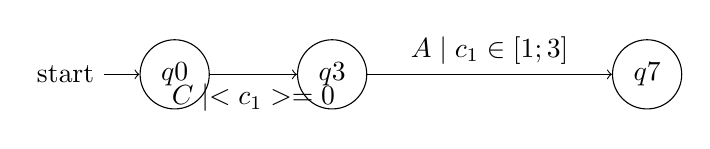
\begin{tikzpicture}[auto]
        \node[state, initial] at (0, 0)(q0){$q0$};
        \node[state] at (2, 0)(q3){$q3$};
        \node[state] at (6, 0)(q7){$q7$};
        
        \path[->]
            (q3)edge node[above]{$A\mid c_1\in[1;3]$}(q7)
            (q0)edge node[below]{$C\mid <c_1>=0$}(q3)
            ;
    \end{tikzpicture}
}

\captionof{figure}{Unreachable states $q4$ and $q2$ have been removed.}
\label{fig:prune3}

\end{frame}
\begin{frame}{Dead state}
    Dead states are all the states that have no way of reaching the final state.
These states are pruned by removing all states that have no edges away from them unless they are final states, this is repeated untill no states satisfy this property.

\sembox{
    $\deadstate(A_1)=\left\{\begin{array}{ll}
        A_1 & if \forall q_1\in Q_1:q_1\notin F_1 \transition[_1]\in\Delta_1 \\
        \deadstate(\automaton[][Q][C_1][\Delta][\Sigma_1][s_1][F_1]) & otherwise \\
    \end{array}\right.
    $

    $Q=\{q_1\in Q_1|q_1\notin F_1\wedge\transition[_1]\in\Delta_1\}$

    $\Delta=\{\transition[_1]\in\Delta_1|q_1\in Q\}$
}
    % Generated by: TimedRegex, Version = 1.0.0.0
% Date 5/14/2024 6:44:16 PM
\usetikzlibrary {automata,positioning}
% "C(A[5;10]&(BA|A)[1;3])"
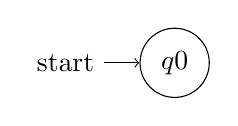
\begin{tikzpicture}[auto]
    \node[state, initial] at (0, 0)(q0){$q0$};
    
    \path[->]
        ;
\end{tikzpicture}
 

\end{frame}
\begin{frame}{Dead clock}
    % Any clocks that are not used in any intervals can be removed.
% This means removing them both from the clocks set and from any clock resets.
% This shouldn't have a huge impact, but it will allow us to create a more minimal declaration field in Uppaal.
\begin{definition}\label{definition:deadClockPruning}
    Dead clock pruning:
    \vspace{0.5em}

    \sembox{
        $\deadclock\automaton=\automaton[][Q][C'][\Delta'][\Sigma][s][F]$

        \vspace{0.5em}

        $C'=\{c\mid\exists\transition[]\in\Delta:\exists(c',I) \in\phi:c=c'\}$

        $\Delta'=\{\transition[][q][q'][\phi][p\cap C']\mid\transition\in\Delta\}$
    }
\end{definition}
    % Generated by: TimedRegex, Version = 1.0.0.0
% Date 5/14/2024 6:44:16 PM
\usetikzlibrary {automata,positioning}
% "C(A[5;10]&(BA|A)[1;3])"
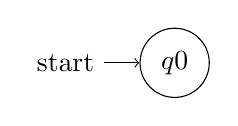
\begin{tikzpicture}[auto]
    \node[state, initial] at (0, 0)(q0){$q0$};
    
    \path[->]
        ;
\end{tikzpicture}
 

\end{frame}
\begin{frame}{Recursion}
    \begin{definition}\label{definition:recursivePruning}
    Recursive pruning:
    
    \sembox{
        $\pruning(A)=\left\{\begin{array}{ll}
            A & \text{if }A=A' \\
        \pruning(A') & otherwise \\
        \end{array}\right.
        $

        $A' = \clockreduction\circ\deadedge\circ\deadstate\circ\unreachable\circ\deadclock(A)$
    }
\end{definition}
    % Generated by: TimedRegex, Version = 1.0.0.0
% Date 5/14/2024 6:44:16 PM
\usetikzlibrary {automata,positioning}
\scalebox{0.9}{
    % "C(A[5;10]&(BA|A)[1;3])"
    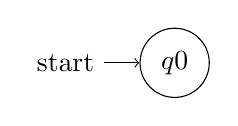
\begin{tikzpicture}[auto]
        \node[state, initial] at (0, 0)(q0){$q0$};
    \end{tikzpicture}
}

\captionof{figure}{Final pruned automaton.}
\label{fig:prune6}

\end{frame}

\begin{frame}{Recursion}
    \begin{definition}\label{definition:recursivePruning}
    Recursive pruning:
    
    \sembox{
        $\pruning(A)=\left\{\begin{array}{ll}
            A & \text{if }A=A' \\
        \pruning(A') & otherwise \\
        \end{array}\right.
        $

        $A' = \clockreduction\circ\deadedge\circ\deadstate\circ\unreachable\circ\deadclock(A)$
    }
\end{definition}
    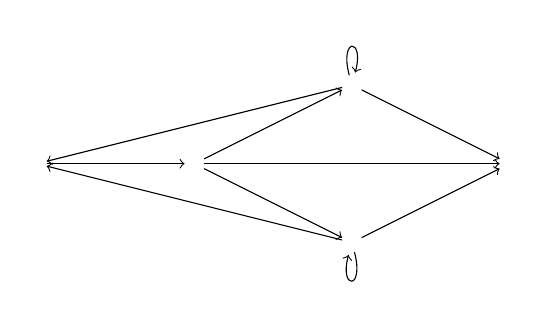
\begin{tikzpicture}[auto]
    \node[] at (0, 0)(cr){$\clockreduction$};
    \node[] at (4, -1)(sd){$\deadstate$};
    \node[] at (4, 1)(su){$\unreachable$};
    \node[] at (2, 0)(td){$\deadedge$};
    \node[] at (6, 0)(cd){$\deadclock$};
    
    \path[->]
        (su)edge [loop above] node{}(su)
        (sd)edge [loop below] node{}(sd)
        (su)edge node[align=left]{}(cr)
        (sd)edge node[align=left]{}(cr)
        (td)edge node[align=left]{}(sd)
        (td)edge node[align=left]{}(su)
        (sd)edge node[align=left]{}(cd)
        (su)edge node[align=left]{}(cd)
        (td)edge node[align=left]{}(cd)
        (cr)edge node[align=left]{}(td)
        ;
\end{tikzpicture}
\end{frame}

% =======================================================================
% Graph layout
% =======================================================================
\section{Graph}
\begin{frame}[shrink=5]{Graph}
    \begin{center}
        \scalebox{0.9}{
    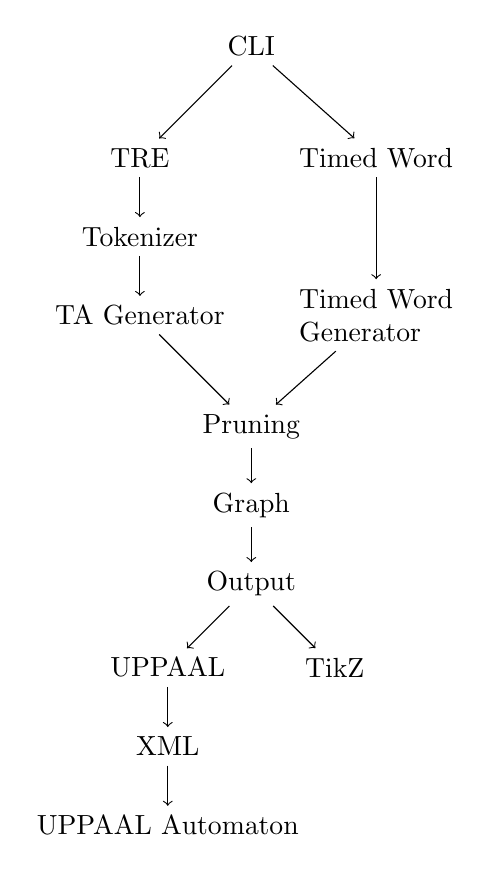
\begin{tikzpicture}[node distance = 1cm, auto]\label{fig:TREATdiagram}
        \node (CLI) {CLI};
        
        \node (TRE) [node distance = 2cm, below left of = CLI] {TRE};
        \node (TimedWord) [node distance = 3cm, right of = TRE] {Timed Word};
        \node (Tokenizer) [below of = TRE] {Tokenizer};
        \node (TAGenerator) [below of = Tokenizer] {TA Generator};
        \node (Pruning) [node distance = 2cm, below right of = TAGenerator] {Pruning};
        \node (Graph) [below of = Pruning] {Graph};
        \node (Output) [below of = Graph] {Output};
        \node (UPPAAL) [node distance = 1.5cm, below left of = Output] {UPPAAL};
        \node (XML) [below of = UPPAAL] {XML};
        \node (UPPAALAutomaton) [below of = XML] {UPPAAL Automaton};
        \node (TikZ) [node distance = 1.5cm, below right of = Output] {TikZ};
        \node (TimedWordGenerator) [node distance = 3cm, right of = TAGenerator,  align=left] {Timed Word\\Generator};
    
        \draw[->] (CLI) -- (TRE);
        \draw[->] (TRE) -- (Tokenizer);
        \draw[->] (Tokenizer) -- (TAGenerator);
        \draw[->] (TAGenerator) -- (Pruning);
        \draw[->] (Pruning) -- (Graph);
        \draw[->] (Graph) -- (Output);
        \draw[->] (Output) -- (UPPAAL);
        \draw[->] (UPPAAL) -- (XML);
        \draw[->] (XML) -- (UPPAALAutomaton);
        \draw[->] (Output) -- (TikZ);
        \draw[->] (CLI) -- (TimedWord);
        \draw[->] (TimedWord) -- (TimedWordGenerator);
        \draw[->] (TimedWordGenerator) -- (Pruning);
    \end{tikzpicture}
}

    \end{center}
\end{frame}
\begin{frame}{Sugiyama Framework}
    We dont need precise algorithm
    \begin{itemize}
        \item Make graph acyclic (trivial)
        \item Assign states to layers
        \item Order states in layers (just needs to be good enough)
        \item Assign positions (simplicity over correctness)
    \end{itemize}
\end{frame}

\begin{frame}[fragile,shrink=5]{Creation of recursive edges}
    \begin{definition}Asarin et al.
        The automaton for $[\![\varphi^+_1 ]\!]$ is $A = (Q_1,C_1,\Sigma,\Delta,s_1,F_1)$ where $\Delta_1$ is constructed from $\Delta_1$ by adding
        for every transition of the form $(q,\varphi,p,a, f_1)$ in $\Delta_1$ with $f_1 \in F_1$ a transition of the form
        $(q,\varphi,C_1,a,s_1)$.
    \end{definition}
        
    \begin{definition}
        Asarin et al.
        The automaton for $[\![\varphi\oplus_1 ]\!]$ is $A = (Q_1 \times 2^{C_1}, C_1 \cup \{x\},\Sigma,\Delta,(s_1,\emptyset),F_1 \times 2^{C_1})$. The second component of the state records which clocks have been reset during the current iteration of $[\![\varphi_1]\!]$.
        There are two types of transitions in $\Delta$:
        \begin{itemize}
            \item Transitions simulating those of $A$ : for every transition of the form $(q,\varphi,p,a,q)$ in $\Delta_1$
            and every $D \subset C_1$ the relation $\Delta$ contains $((q,D),\varphi_D,p,a,(q',D\cup p))$
            \item Looping transitions: for every transition of the form $(q_1,\varphi,p,a, f_1)$ in $\Delta_1$ with $f_1 \in F_1$ and
            every $D \subset C_1$ the relation $\Delta$ contains $((q_1,D),\varphi_D,p,a,(s_1,\emptyset))$.
        \end{itemize}
        Here $\varphi_D$ is obtained by replacing in $\varphi$ all occurrences of clocks not belonging to $D$ by $x$
    \end{definition}
\end{frame}
    
\begin{frame}[fragile]{Keeping reversible edges (1)}
    \begin{definition}
        Asarin et al.
        The automaton for $[\![\varphi\oplus_1 ]\!]$ is $A = (Q_1 \times 2^{C_1}, C_1 \cup \{x\},\Sigma,\Delta,(s_1,\emptyset),F_1 \times 2^{C_1})$. The second component of the state records which clocks have been reset during the current iteration of $[\![\varphi_1]\!]$.
        There are two types of transitions in $\Delta$:
        \begin{itemize}
            \item Transitions simulating those of $A$ : for every transition of the form $(q,\varphi,p,a,q)$ in $\Delta_1$
            and every $D \subset C_1$ the relation $\Delta$ contains $((q,D),\varphi_D,p,a,(q',D\cup p))$
            \item Looping transitions: for every transition of the form $(q_1,\varphi,p,a, f_1)$ in $\Delta_1$ with $f_1 \in F_1$ and
            every $D \subset C_1$ the relation $\Delta$ contains $((q_1,D),\varphi_D,p,a,(s_1,\emptyset))$.
        \end{itemize}
        Here $\varphi_D$ is obtained by replacing in $\varphi$ all occurrences of clocks not belonging to $D$ by $x$
    \end{definition}
\end{frame}
\begin{frame}[fragile]{Keeping reversible edges (2)}
    \begin{definition}
        The automaton for $[\![\varphi_1\wedge\varphi_2]\!]$ is $(Q_1\times Q_2 \cup \{f\}, C_1\cup C_2,\Delta,\Sigma,(s_1,s_2),\{f\})$, where $\Delta$ contains
        \begin{itemize}
            \item a transition $\{((q_1,q_2),\Phi_1\wedge\Phi_2,p_1\cup p_2, a, (q'_1,q'_2))$for any$(q_1,\Phi_1,p_1,a,q'_1)\in\Delta_1$and any$(q_2,\Phi_2,p_2,a,q'_2)\in\Delta_2\}$;
            \item a transition $\{((q_1,q_2),\Phi_1\wedge\Phi_2,p_1\cup p_2, a, f)$for any$(q_1,\Phi_1,p_1,a,f'_1)\in\Delta_1$and any$(q_2,\Phi_2,p_2,a,f'_2)\in\Delta_2\}$ where $f_1\in F_1$ and $f_2\in F_2$;
            \item a transition $\{((q_1,q_2),\Phi_1,p_1,\epsilon,(q'_1,q))$for any$(q_1,\Phi_1,p_1,\epsilon,q'_1)\in\Delta_1\}$;
            \item a transition $\{((q_1,q_2),\Phi_2,p_2,\epsilon,(q,q'_2))$for any$(q_2,\Phi_2,p_2,\epsilon,q'_2)\in\Delta_2\}$;
        \end{itemize}
    \end{definition}

    % \begin{lstlisting}[style=csharp,basicstyle=\tiny]
    %     State GetNewState(State lState, State rState)
    %     {
    %         if (!newLocs.TryGetValue((lState, rState), out State? state))
    %         {
    %             state = ta.AddState();
    %             newLocs[(lState, rState)] = state;
    %         }
        
    %         return state;
    %     }
    % \end{lstlisting}
\end{frame}

\begin{frame}[fragile]{Removing recursive edges}
    In graphlayout
    \begin{lstlisting}[style=csharp,basicstyle=\tiny]
private void AssignLayers(TimedAutomaton ta, TaState taState, int layerIndex)
...
foreach (Edge edge in ta.GetEdgesFrom(taState)
    .Where(e => !e.IsReversible))
    ...
foreach (Edge edge in ta.GetEdgesTo(taState)
    .Where(e => e.IsReversible && !e.To.Equals(taState)))
    ...
...
    \end{lstlisting}
\end{frame}

\renewcommand{\name}{Emil}
\section{UPPAAL}
\begin{frame}{UPPAAL}
    \begin{columns}
        \begin{column}{0.4\textwidth}
            \begin{itemize}
                \item UML
                \item Structured using UPPAAL .dtd
            \end{itemize}
        \end{column}
        \begin{column}{0.6\textwidth}
            \scalebox{0.8}{
                \scalebox{0.8}{
\begin{tikzpicture}
        \umlclass[anchor=north,width=31ex,x=0,y=0]{nta}{declaration : string\\system : string}{}

        %classes
        \umlclass[anchor=north,width=31ex,x=0,y=-4.3]{template}{declaration : string\\name : string\\ init : string}{}
        %relations
        \umlcompo[attr1=1|,attr2=0..*|,pos2=0.87]{nta}{template}

        %classes
        %\umlclass[x=-6,y=-6]{parameter}{}{}
        %\umlclass[x=-3,y=-6]{branchpoint}{}{}
        \umlclass[anchor=north,width=31ex,x=0,y=-9]{location}{id : string\\name : string\\label : List$<$(string, string)$>$}{}
        \umlclass[anchor=north,width=31ex,x=6,y=-9]{transition}{id : string\\source : string\\target : string\\label : List$<$(string, string)$>$}{}
        %\umlclass[x=15,y=-6]{parameter}{}{}
        %relations
        \umlcompo[attr1=1|,attr2=0..*|,pos1=0.15,pos2=0.9]{template}{location}
        \umlHVcompo[attr1=1|,attr2=0..*|,pos1=0.1,pos2=1.95]{template}{transition}
        %\umlVHVcompo[attr2=0..1|,pos2=2.75]{template}{parameter}

        %classes
        %\umlclass[x=-6,y=-9]{committed}{}{}
        %\umlclass[x=-9,y=-9]{urgent}{}{}
        %relations
        %\umlVHVcompo[attr2=0..1|,pos2=2.75]{location}{committed}
        %\umlVHVcompo[attr2=0..1|,pos2=2.75]{location}{urgent}
    \end{tikzpicture}}


            }
        \end{column}
    \end{columns}
    % \hspace{10em}

\end{frame}
\begin{frame}[fragile]{UPPAAL}
    \definecolor{bluekeywords}{rgb}{0,0,1}
    \definecolor{greencomments}{rgb}{0,0.5,0}
    \definecolor{redstrings}{rgb}{0.64,0.08,0.08}
    \definecolor{xmlcomments}{rgb}{0.5,0.5,0.5}
    \definecolor{types}{rgb}{0.17,0.57,0.68}

    \lstset{language=[Sharp]C,
        captionpos=b,
        %numbers=left, %Nummerierung
        %numberstyle=\tiny, % kleine Zeilennummern
        frame=lines, % Oberhalb und unterhalb des Listings ist eine Linie
        showspaces=false,
        showtabs=false,
        breaklines=true,
        showstringspaces=false,
        breakatwhitespace=true,
        commentstyle=\color{greencomments},
        morekeywords={partial, var, value, get, set},
        keywordstyle=\color{bluekeywords},
        stringstyle=\color{redstrings},
        basicstyle=\ttfamily\tiny,
    }
    \begin{lstlisting}
internal Nta()
{
    _templates = new List<Template>();
    Declaration = new Declaration(new List<string>(), new List<string>());
}    
    \end{lstlisting}
    \vspace{1em}
    \begin{lstlisting}
internal Template(...)
{
    Declaration = declaration;
    Declaration.AddClocks(clocks);
    Name = name;
    Init = init;
    _locations = locations.ToArray();
    _transitions = transitions.ToArray();
}  
    \end{lstlisting}
\end{frame}

\begin{frame}{Demonstration}

\end{frame}

\section{Discussion}
\begin{frame}{Future works}
    \begin{columns}
        \begin{column}{0.4\textwidth}
            \begin{itemize}
                \item Pruning
                \item <4>TA $\rightarrow$ TRE
            \end{itemize}
        \end{column}
        \begin{column}{0.6\textwidth}
            \visible<2-3> {
                \scalebox{0.8}{
                    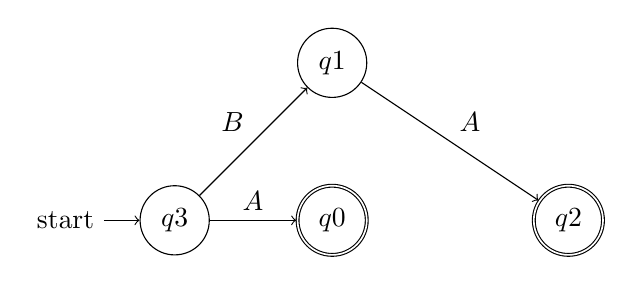
\begin{tikzpicture}[auto]
                        \node[state, accepting] at (2, 0)(q0){$q0$};
                        \node[state] at (2, 2)(q1){$q1$};
                        \node[state, accepting] at (5, 0)(q2){$q2$};
                        \node[state, initial] at (0, 0)(q3){$q3$};

                        \path[->]
                        (q1)edge node{$A$}(q2)
                        (q3)edge node{$A$}(q0)
                        (q3)edge node{$B$}(q1)
                        ;
                    \end{tikzpicture}
                }
            }

            \vspace{2em}
            \visible<3> {
                \scalebox{0.8}{
                    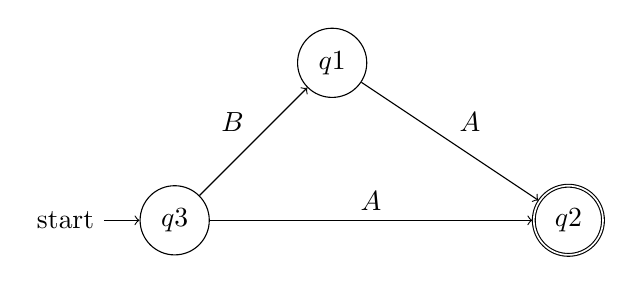
\begin{tikzpicture}[auto]
                        \node[state, accepting] at (5, 0)(q2){$q2$};
                        \node[state] at (2, 2)(q1){$q1$};
                        \node[state, initial] at (0, 0)(q3){$q3$};

                        \path[->]
                        (q1)edge node{$A$}(q2)
                        (q3)edge node{$A$}(q2)
                        (q3)edge node{$B$}(q1)
                        ;
                    \end{tikzpicture}
                }
            }
        \end{column}
    \end{columns}
\end{frame}
\begin{frame}{Enhancements}
    \begin{itemize}
        \item Bugfixes after hand-in
              \begin{itemize}
                  \item int32 indices
                  \item graph layout crashes
                  \item $\cdots$
              \end{itemize}
    \end{itemize}

\end{frame}
\begin{frame}{Learning Goals}
    \begin{itemize}
        \item is this relevant? genuine question
    \end{itemize}
\end{frame}
\section{Conclusion}
\begin{frame}{Conclusion}
    \begin{itemize}
        \item TREAT
        \item Readability
    \end{itemize}
\end{frame}

\end{document}